
\begin{figure}
\centering
\begin{subfigure}{.5\textwidth}
  \centering
  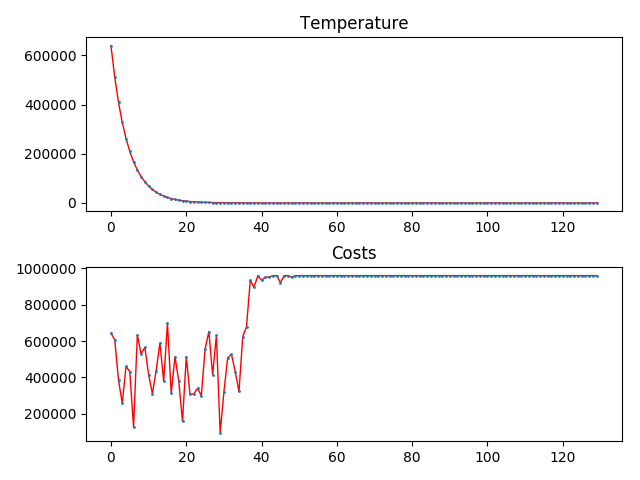
\includegraphics[width=1\linewidth]{results/cut12/2/plot}
  \label{fig:sub1}
\end{subfigure}%
\begin{subfigure}{.5\textwidth}
  \centering
  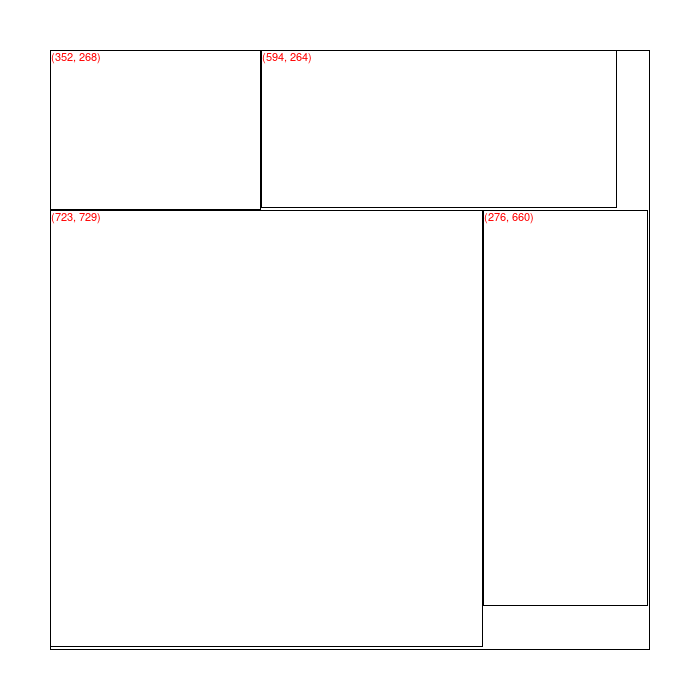
\includegraphics[width=1\linewidth]{results/cut12/2/cut}
  \label{fig:sub2}
\end{subfigure}
\caption{Instancia cut12.txt, Solução: 911260, desperdício de 8.87\% de 1000x1000, {(268, 352): 1, (264, 594): 1, (566, 349): 1, (734, 616): 1}}
\label{fig:test}
\end{figure}


\begin{figure}
\centering
\begin{subfigure}{.5\textwidth}
  \centering
  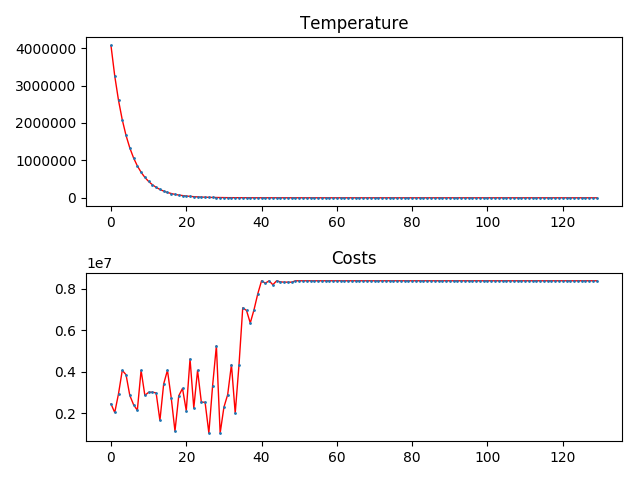
\includegraphics[width=1\linewidth]{results/cut13/1/plot}
  \label{fig:sub1}
\end{subfigure}%
\begin{subfigure}{.5\textwidth}
  \centering
  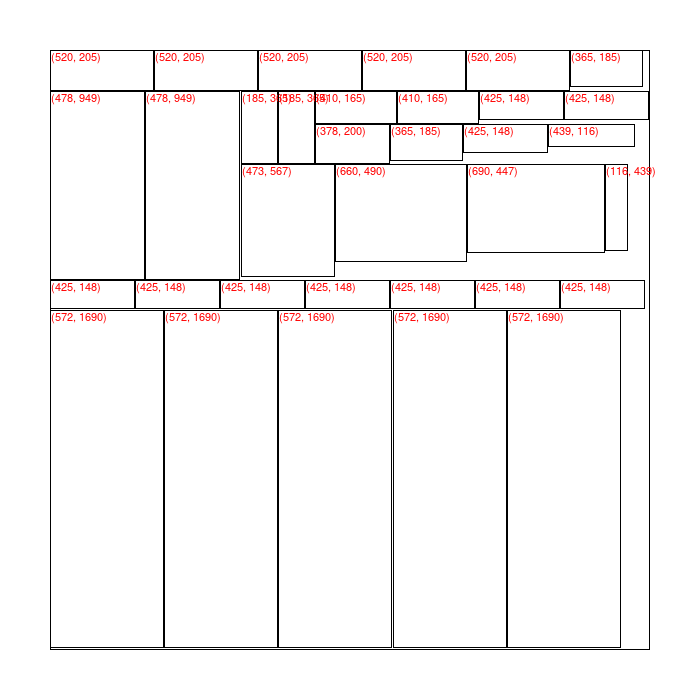
\includegraphics[width=1\linewidth]{results/cut13/1/cut}
  \label{fig:sub2}
\end{subfigure}
\caption{Instancia cut13.txt, Solução: 8385513, desperdício de 6.83\% de 3000x3000, {(296, 425): 2, (1890, 572): 1, (572, 1890): 2, (365, 185): 2, (425, 296): 1, (350, 520): 1, (949, 445): 1, (439, 116): 1, (378, 200): 2, (410, 165): 1, (165, 410): 1, (205, 520): 2, (690, 447): 1, (549, 1882): 1, (572, 1575): 2}}
\label{fig:test}
\end{figure}


\begin{figure}
\centering
\begin{subfigure}{.5\textwidth}
  \centering
  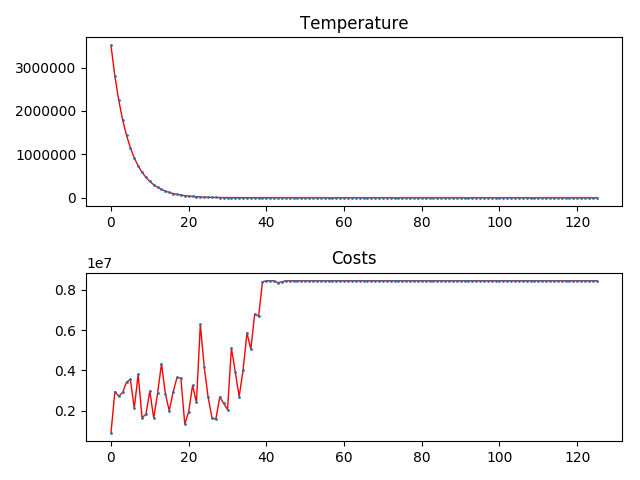
\includegraphics[width=1\linewidth]{results/cut14/2/plot}
  \label{fig:sub1}
\end{subfigure}%
\begin{subfigure}{.5\textwidth}
  \centering
  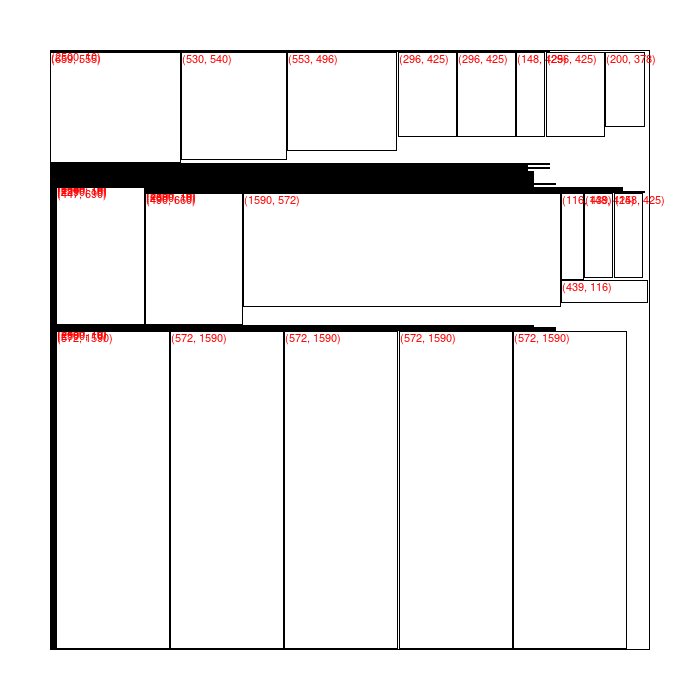
\includegraphics[width=1\linewidth]{results/cut14/2/cut}
  \label{fig:sub2}
\end{subfigure}
\caption{Instancia cut14.txt, Solução: 8817124, desperdício de 2.03\% de 3000x3000, {(2500, 10): 2, (520, 205): 2, (425, 148): 1, (572, 592): 1, (439, 116): 1, (949, 445): 1, (200, 378): 1, (949, 478): 2, (378, 200): 4, (410, 165): 3, (205, 520): 1, (572, 1690): 5, (2390, 10): 3, (755, 555): 1, (473, 567): 1}}
\label{fig:test}
\end{figure}


\begin{figure}
\centering
\begin{subfigure}{.5\textwidth}
  \centering
  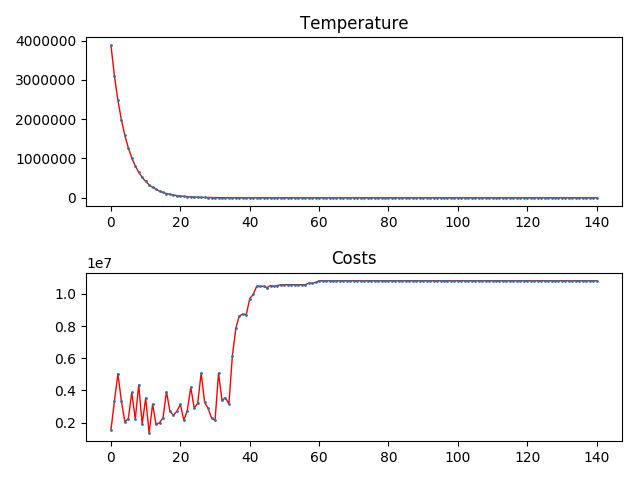
\includegraphics[width=1\linewidth]{results/cut17/3/plot}
  \label{fig:sub1}
\end{subfigure}%
\begin{subfigure}{.5\textwidth}
  \centering
  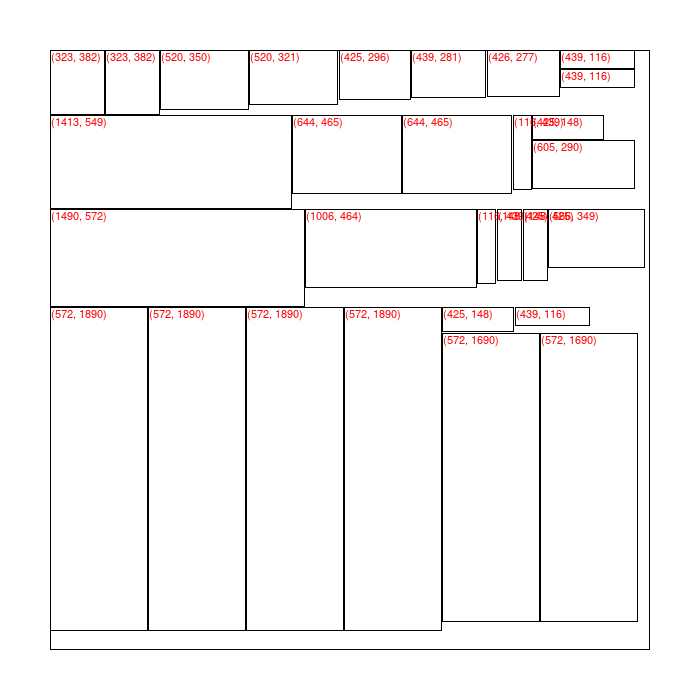
\includegraphics[width=1\linewidth]{results/cut17/3/cut}
  \label{fig:sub2}
\end{subfigure}
\caption{Instancia cut17.txt, Solução: 11264909, desperdício de 8.04\% de 3500x3500, {(1390, 572): 2, (526, 273): 1, (268, 352): 1, (483, 532): 1, (446, 327): 2, (640, 482): 1, (439, 281): 1, (116, 439): 1, (425, 148): 1, (417, 300): 1, (656, 278): 1, (365, 185): 1, (323, 382): 1, (659, 555): 1, (572, 1890): 6, (519, 604): 1, (546, 590): 1, (200, 378): 1, (414, 678): 1}}
\label{fig:test}
\end{figure}


\begin{figure}
\centering
\begin{subfigure}{.5\textwidth}
  \centering
  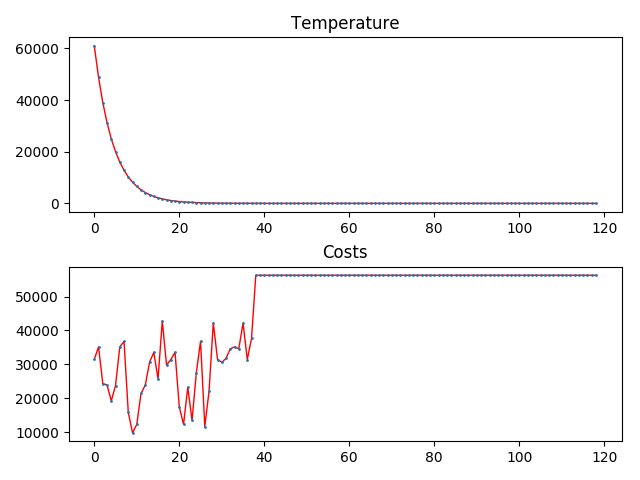
\includegraphics[width=1\linewidth]{results/cut1/1/plot}
  \label{fig:sub1}
\end{subfigure}%
\begin{subfigure}{.5\textwidth}
  \centering
  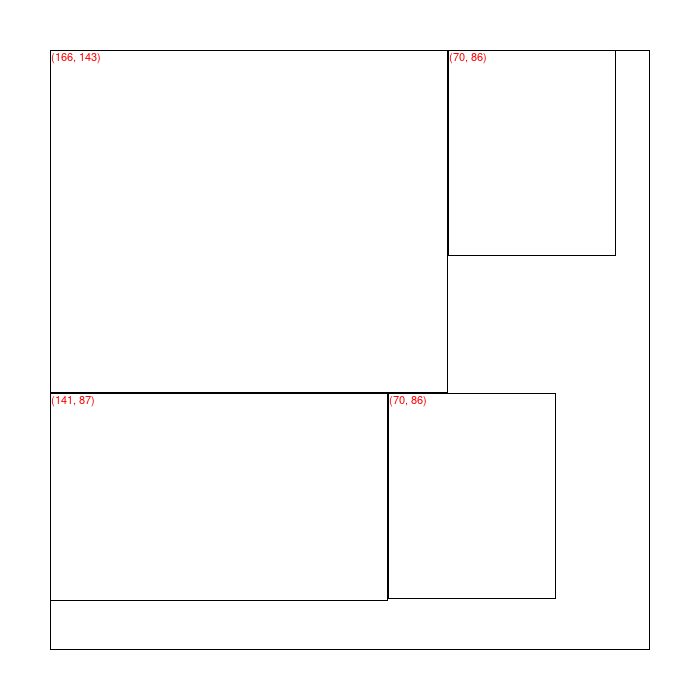
\includegraphics[width=1\linewidth]{results/cut1/1/cut}
  \label{fig:sub2}
\end{subfigure}
\caption{Instancia cut1.txt, Solução: 58136, desperdício de 6.98\% de 250x250, {(148, 66): 1, (66, 148): 1, (184, 167): 1, (86, 70): 1}}
\label{fig:test}
\end{figure}


\begin{figure}
\centering
\begin{subfigure}{.5\textwidth}
  \centering
  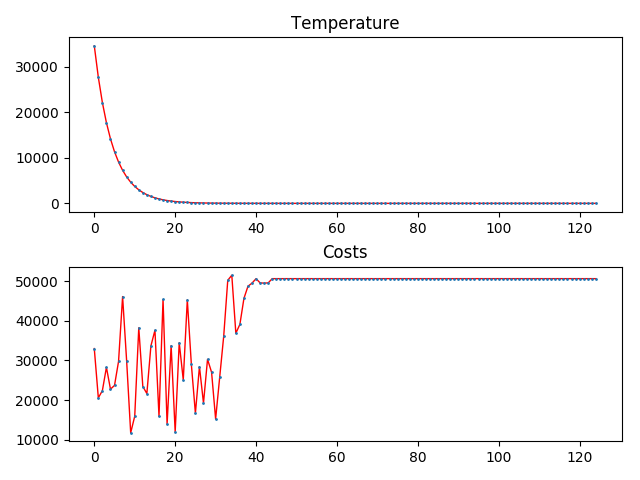
\includegraphics[width=1\linewidth]{results/cut2/2/plot}
  \label{fig:sub1}
\end{subfigure}%
\begin{subfigure}{.5\textwidth}
  \centering
  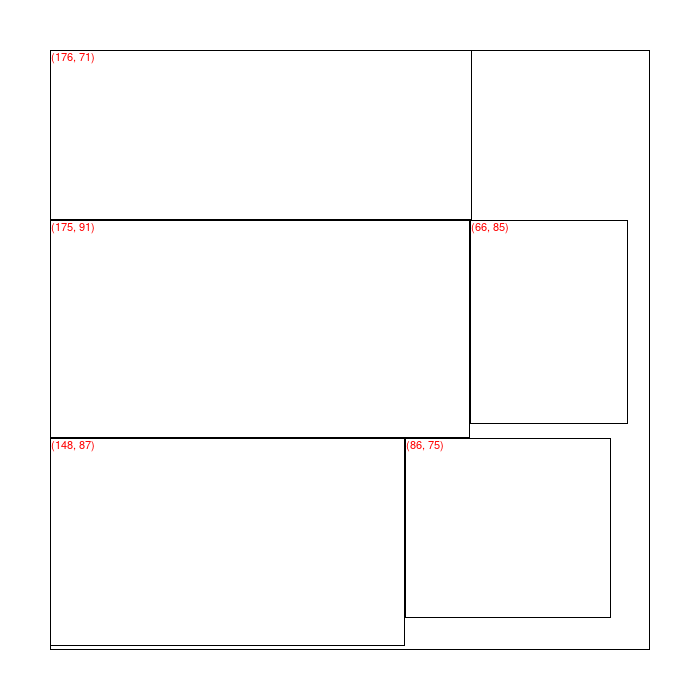
\includegraphics[width=1\linewidth]{results/cut2/2/cut}
  \label{fig:sub2}
\end{subfigure}
\caption{Instancia cut2.txt, Solução: 56604, desperdício de 9.43\% de 250x250, {(186, 135): 1, (168, 107): 1, (73, 103): 1}}
\label{fig:test}
\end{figure}


\begin{figure}
\centering
\begin{subfigure}{.5\textwidth}
  \centering
  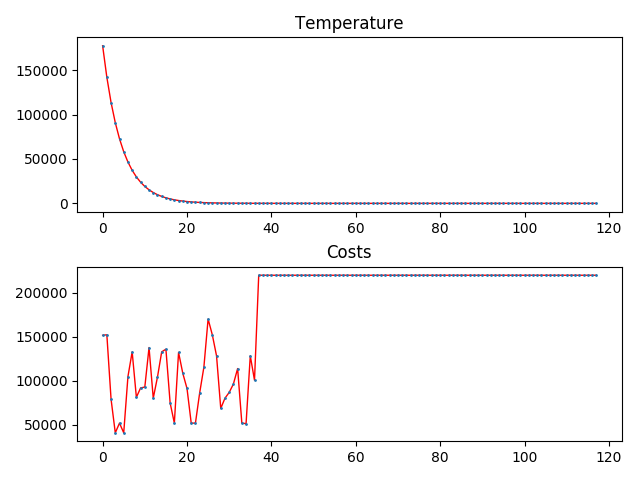
\includegraphics[width=1\linewidth]{results/cut5/3/plot}
  \label{fig:sub1}
\end{subfigure}%
\begin{subfigure}{.5\textwidth}
  \centering
  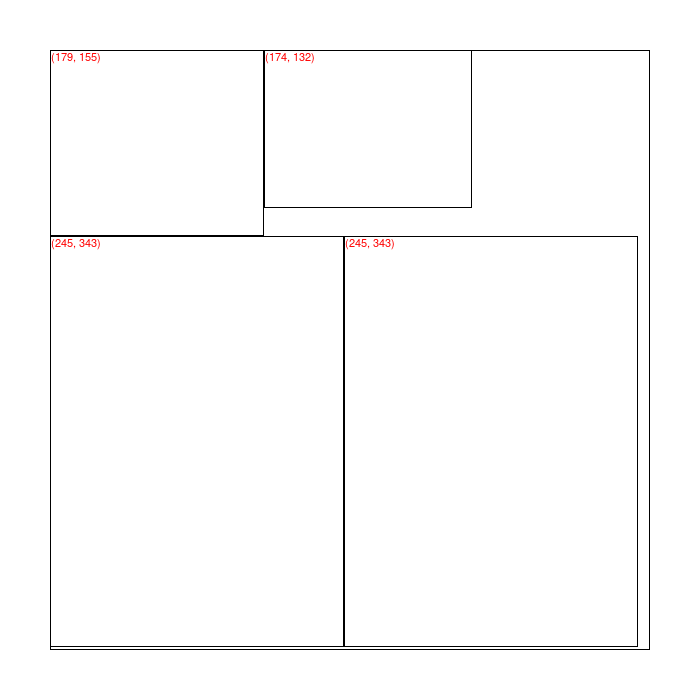
\includegraphics[width=1\linewidth]{results/cut5/3/cut}
  \label{fig:sub2}
\end{subfigure}
\caption{Instancia cut5.txt, Solução: 218783, desperdício de 12.49\% de 500x500, {(174, 132): 1, (245, 343): 2, (179, 155): 1}}
\label{fig:test}
\end{figure}


\begin{figure}
\centering
\begin{subfigure}{.5\textwidth}
  \centering
  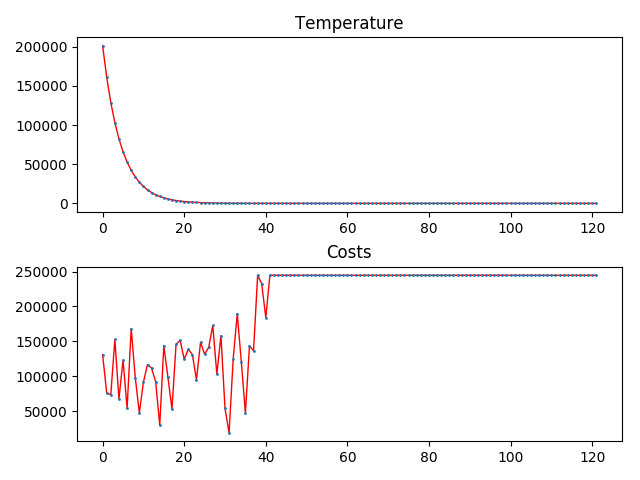
\includegraphics[width=1\linewidth]{results/cut7/3/plot}
  \label{fig:sub1}
\end{subfigure}%
\begin{subfigure}{.5\textwidth}
  \centering
  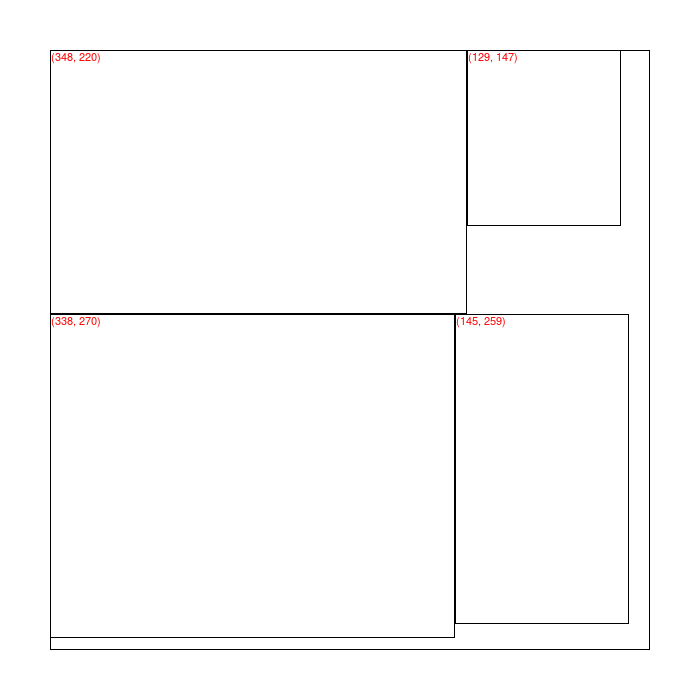
\includegraphics[width=1\linewidth]{results/cut7/3/cut}
  \label{fig:sub2}
\end{subfigure}
\caption{Instancia cut7.txt, Solução: 237543, desperdício de 4.98\% de 500x500, {(146, 351): 1, (198, 129): 1, (259, 145): 1, (350, 352): 1}}
\label{fig:test}
\end{figure}


\begin{figure}
\centering
\begin{subfigure}{.5\textwidth}
  \centering
  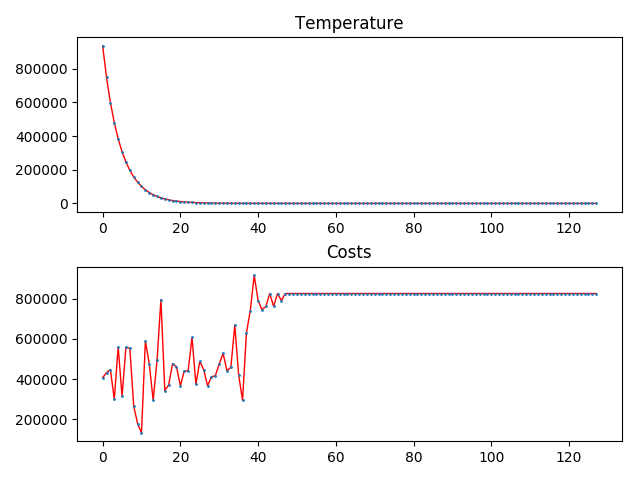
\includegraphics[width=1\linewidth]{results/cut9/2/plot}
  \label{fig:sub1}
\end{subfigure}%
\begin{subfigure}{.5\textwidth}
  \centering
  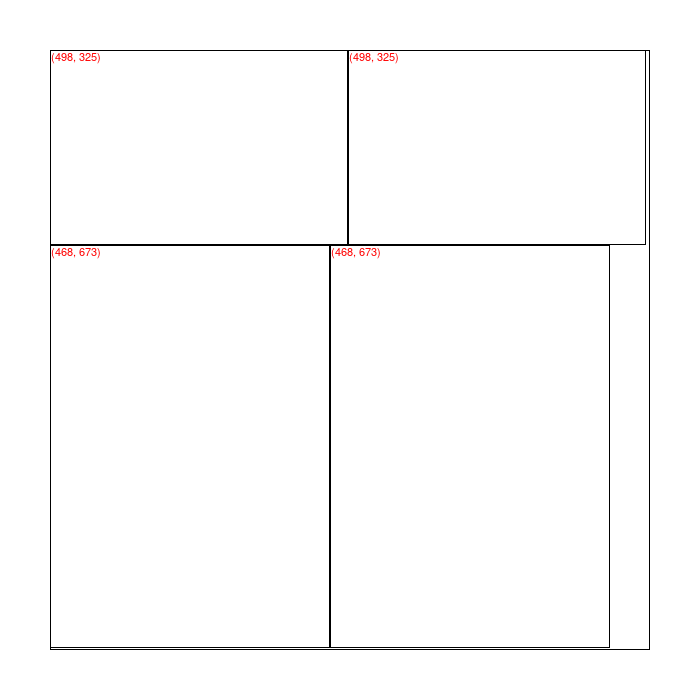
\includegraphics[width=1\linewidth]{results/cut9/2/cut}
  \label{fig:sub2}
\end{subfigure}
\caption{Instancia cut9.txt, Solução: 826236, desperdício de 17.38\% de 1000x1000, {(426, 463): 1, (310, 426): 1, (555, 540): 1, (463, 426): 1}}
\label{fig:test}
\end{figure}


\begin{figure}
\centering
\begin{subfigure}{.5\textwidth}
  \centering
  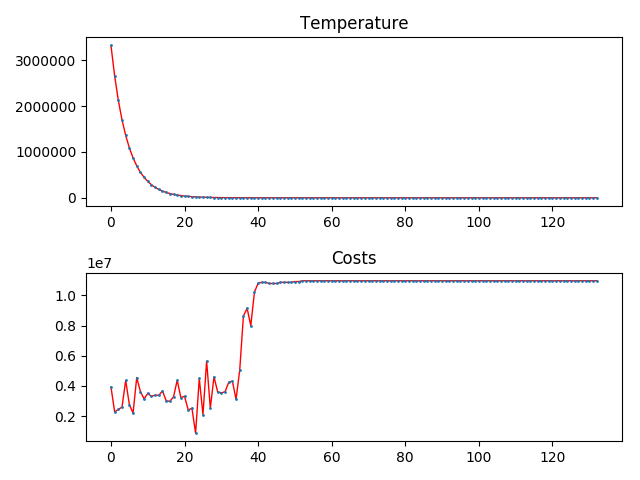
\includegraphics[width=1\linewidth]{results/livre/1/plot}
  \label{fig:sub1}
\end{subfigure}%
\begin{subfigure}{.5\textwidth}
  \centering
  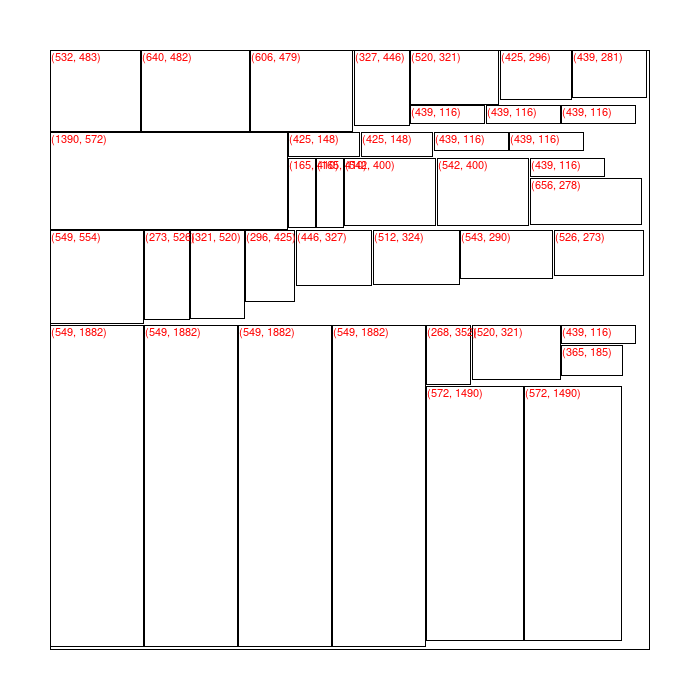
\includegraphics[width=1\linewidth]{results/livre/1/cut}
  \label{fig:sub2}
\end{subfigure}
\caption{Instancia livre.txt, Solução: 11489001, desperdício de 6.21\% de 3500x3500, {(526, 273): 1, (520, 205): 2, (572, 1590): 6, (949, 445): 1, (970, 463): 1, (679, 467): 1, (572, 975): 1, (300, 417): 1, (446, 327): 1, (439, 116): 2, (116, 439): 2, (425, 148): 4, (378, 200): 2, (290, 543): 1, (365, 185): 4, (410, 165): 2, (323, 382): 1, (520, 321): 2, (327, 446): 1, (1575, 572): 1, (200, 378): 1, (665, 572): 1, (339, 405): 1}}
\label{fig:test}
\end{figure}

